\chapter{运动控制仿真}\label{chap:control_simulation}
\section{仿真环境与工具选择}
为了验证前一章设计的控制方案的有效性，我们选择了MATLAB/Simulink作为仿真平台。MATLAB提供了强大的数值计算能力和丰富的工具箱，Simulink则支持基于模型的设计和仿真，能够直观地构建系统模型并进行动态仿真。此外，我们还利用了Simscape Multibody模块来建立机器人动力学模型，并使用Reinforcement Learning Toolbox来实现基于深度强化学习的路径规划算法。
\section{控制方案仿真设计}
仿真设计分为以下几个步骤：

1）建立机器人动力学模型：基于前一章的建模结果，我们在Simscape Multibody中构建了轮腿式机器人的动力学模型，包含底盘、腿部结构以及轮子等关键组件。

2）实现控制算法：根据前一章设计的控制方案，我们在Simulink中实现了相应的控制算法，从LQR输出腿部等效力和力矩，再通过VMC转化到轮电机和关节电机的控制输入。

3）设置仿真场景：为了测试控制方案的性能，本毕业设计设计了多个仿真场景，包括平坦地面、带有障碍物的环境，以评估机器人在不同环境下的运动控制能力。

4）运行仿真并收集数据：通过运行仿真，我们收集了机器人在不同场景下的电机控制输入和状态量的输出数据。

\section{控制框架设计}
\begin{figure}[H]
  \centering
  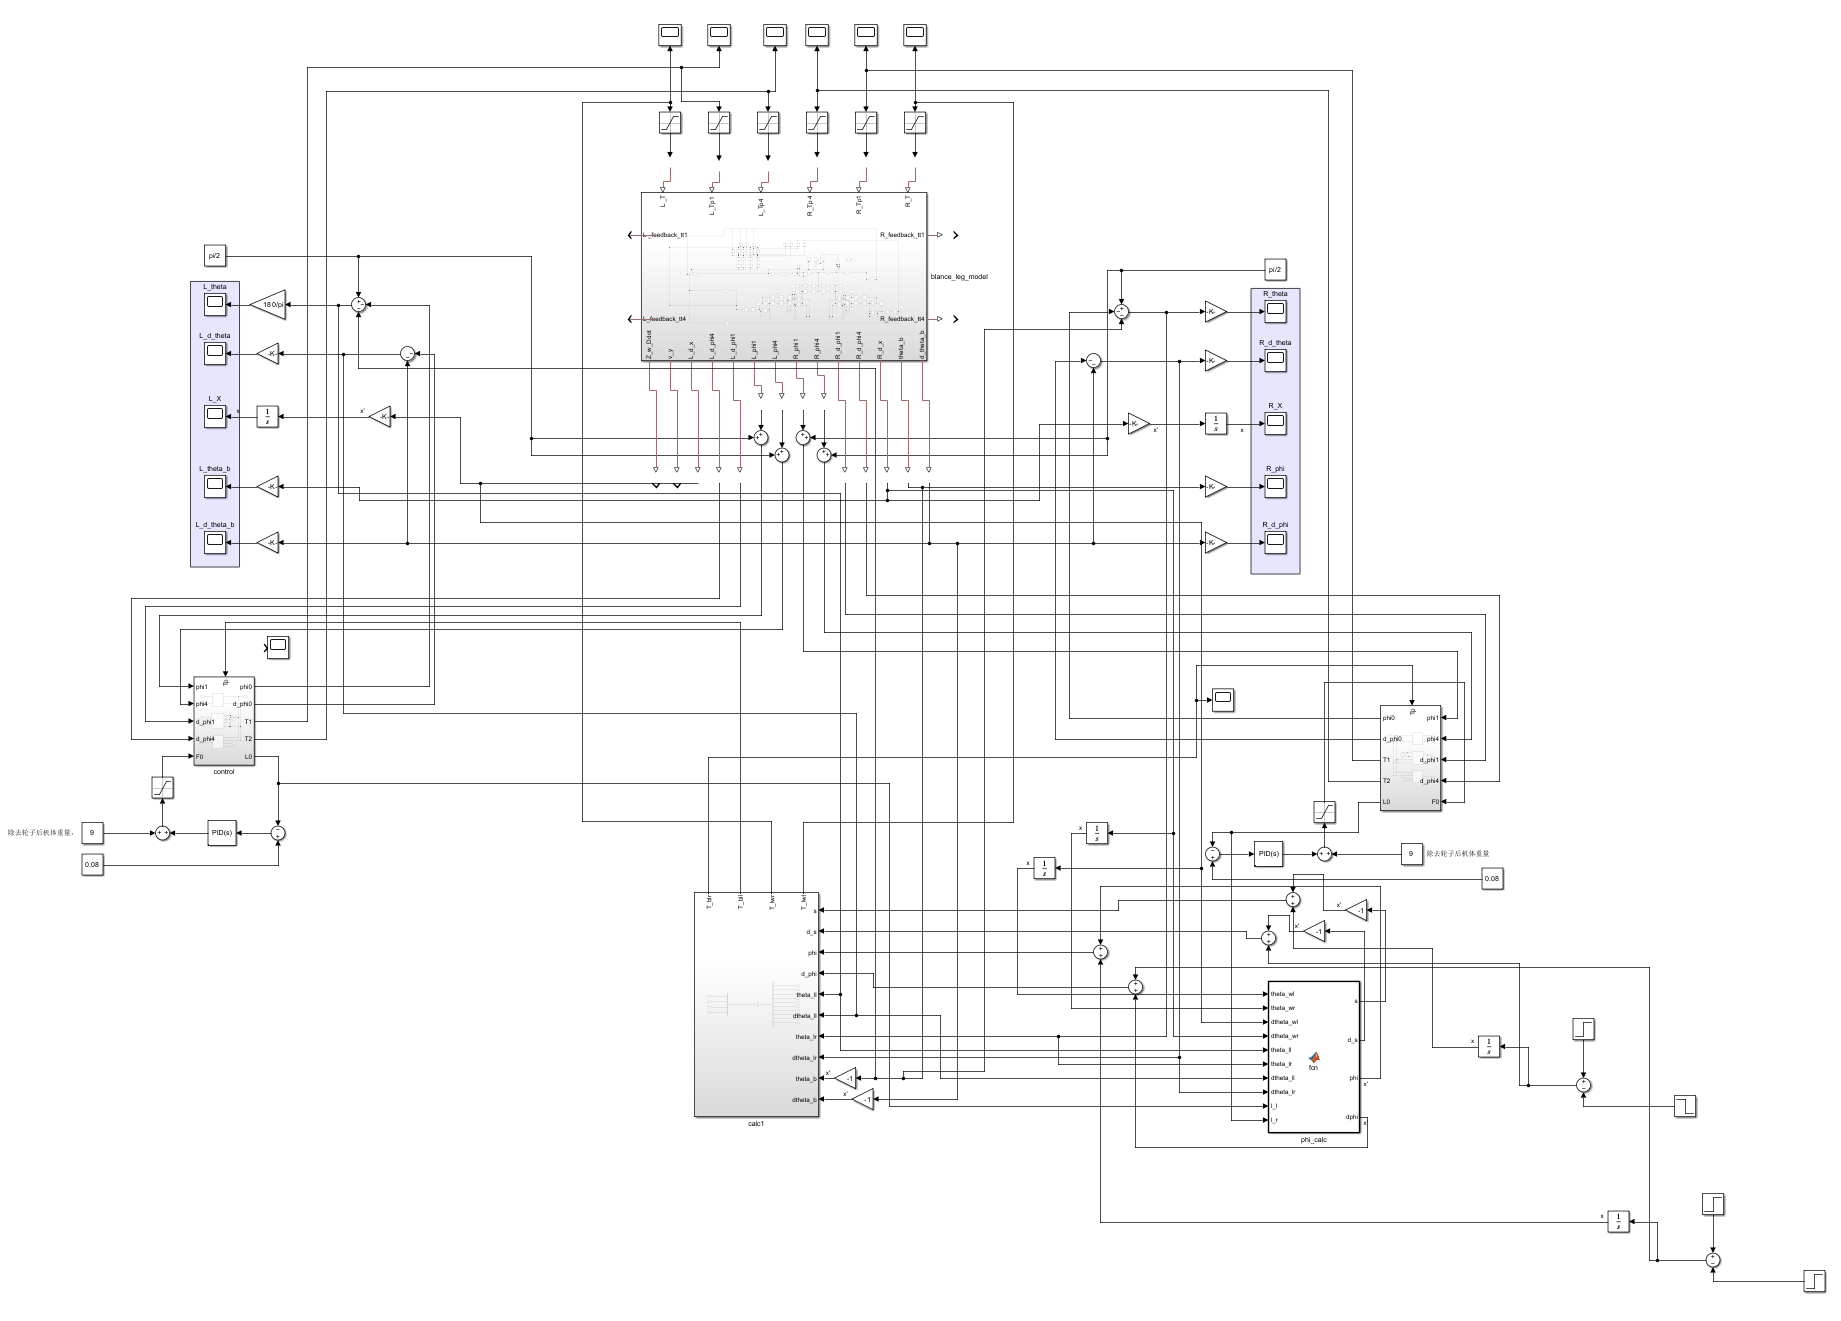
\includegraphics[width=0.9\textwidth]{figures/control_framework.png}
  \caption{控制框架设计}
  \label{fig:control-framework}
\end{figure}
在simulink中搭建了一个控制框架，如图\ref{fig:control-framework}所示。该框架包括以下几个模块：
\subsection{仿真环境搭建}
\begin{figure}[H]
  \centering
  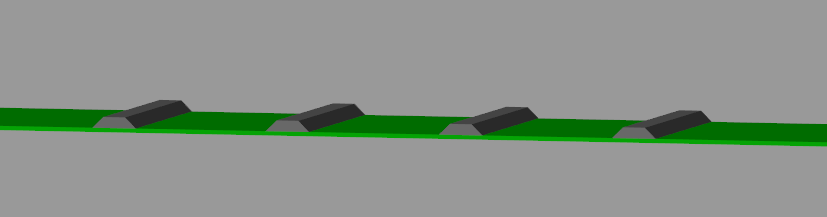
\includegraphics[width=0.9\textwidth]{figures/simulink_env.png}
  \caption{仿真环境搭建}
  \label{fig:simulation-environment}
\end{figure}

\begin{figure}[H]
  \centering
  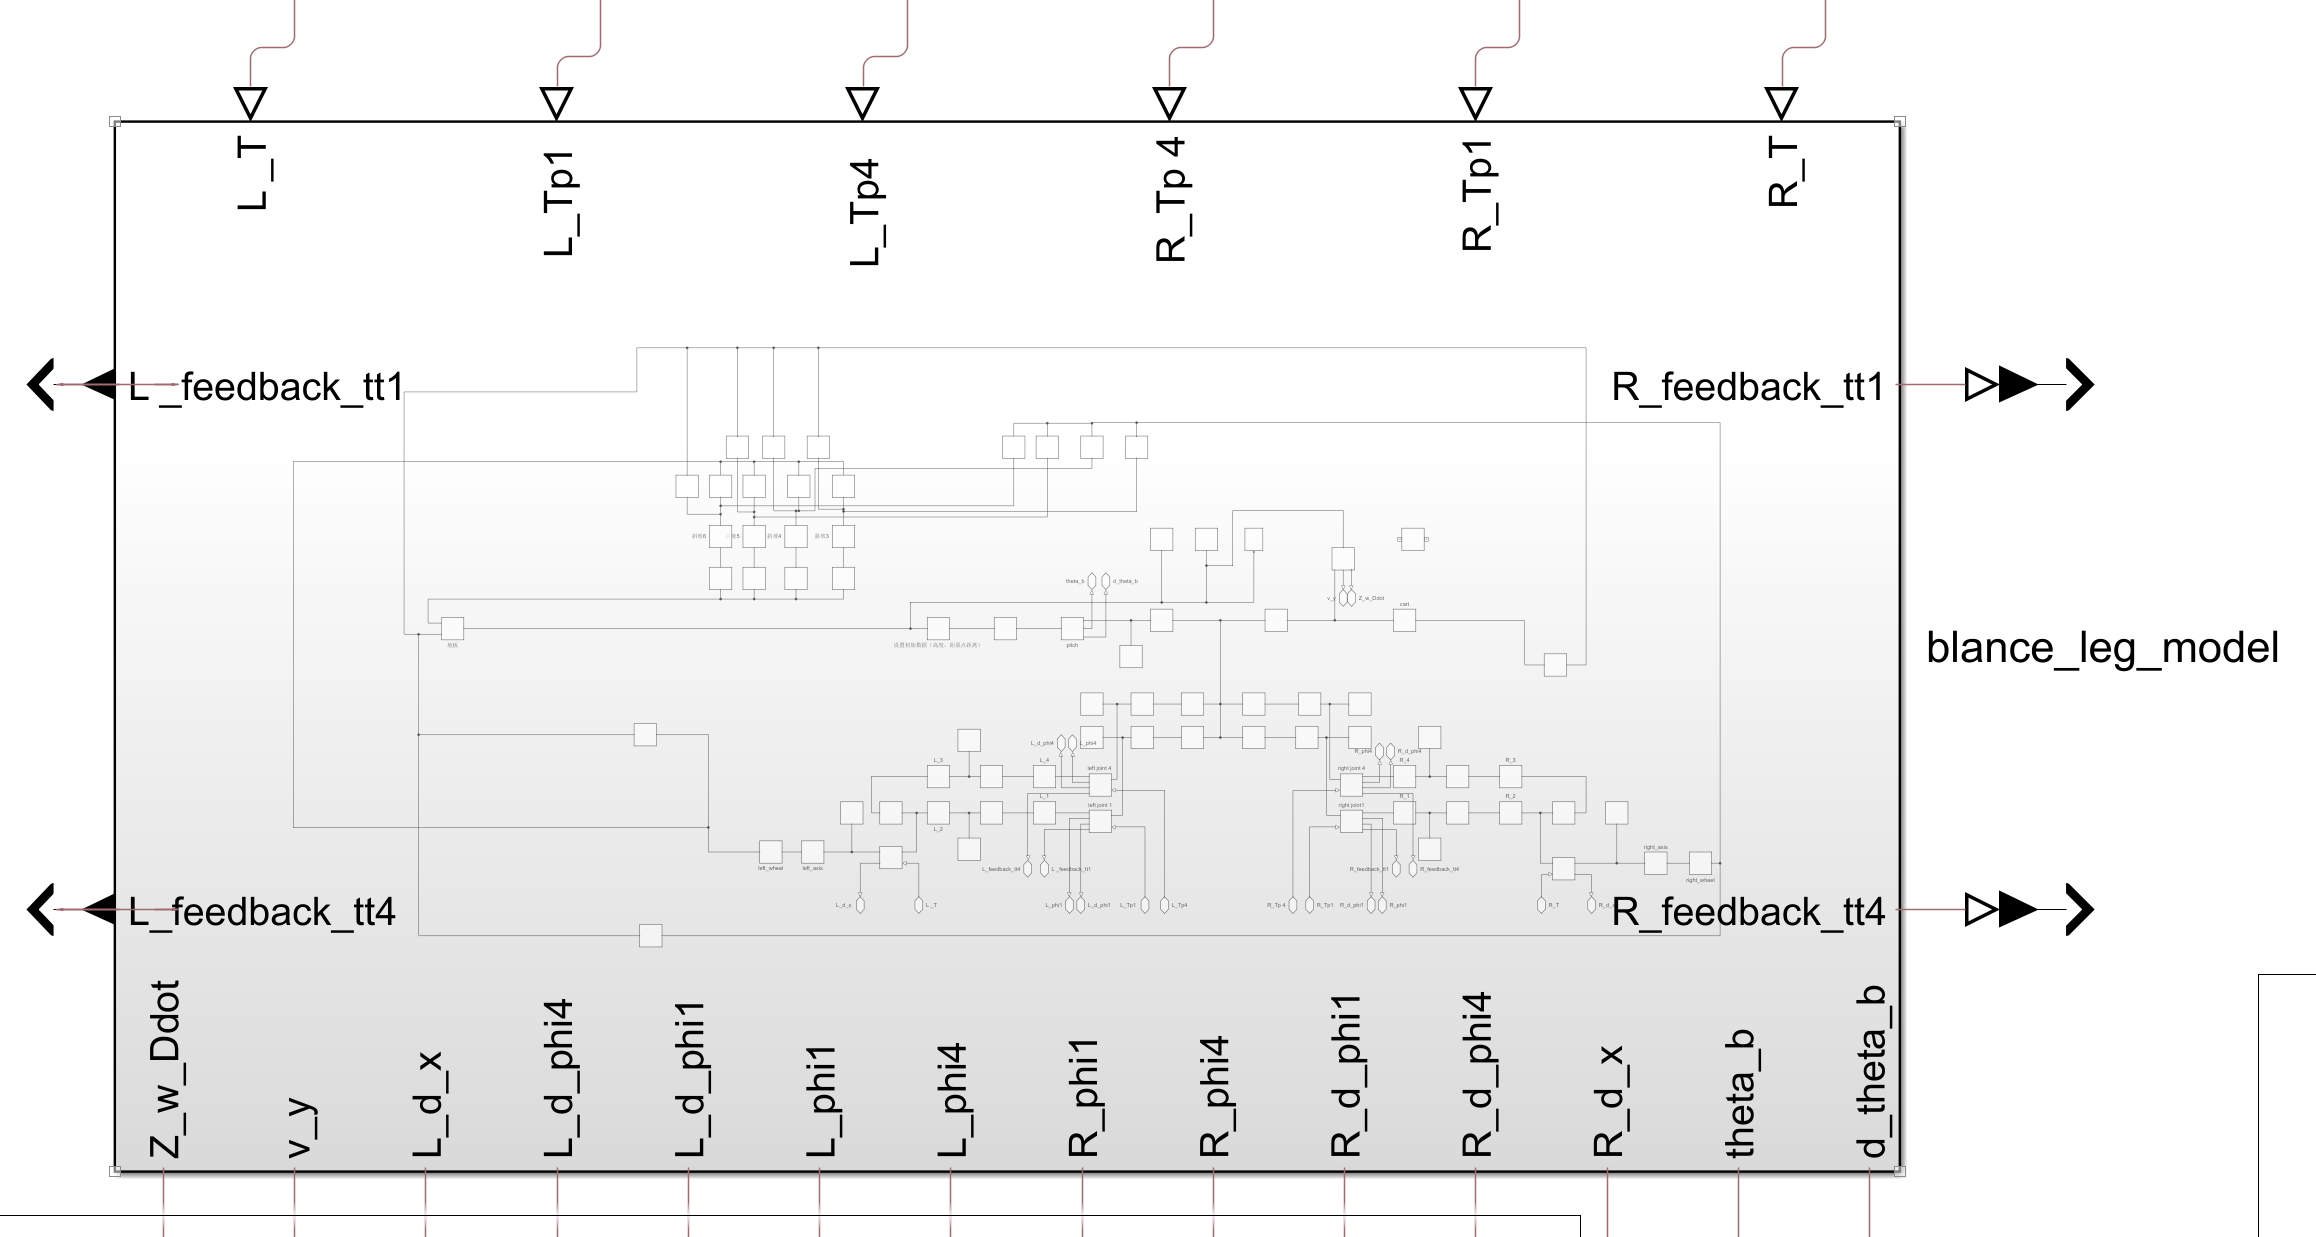
\includegraphics[width=0.7\textwidth]{figures/model_simulink_outside.png}
  \caption{轮腿机器人建模外部接口}
  \label{fig:model-simulink-outside}
\end{figure}

\begin{figure}[H]
  \centering
  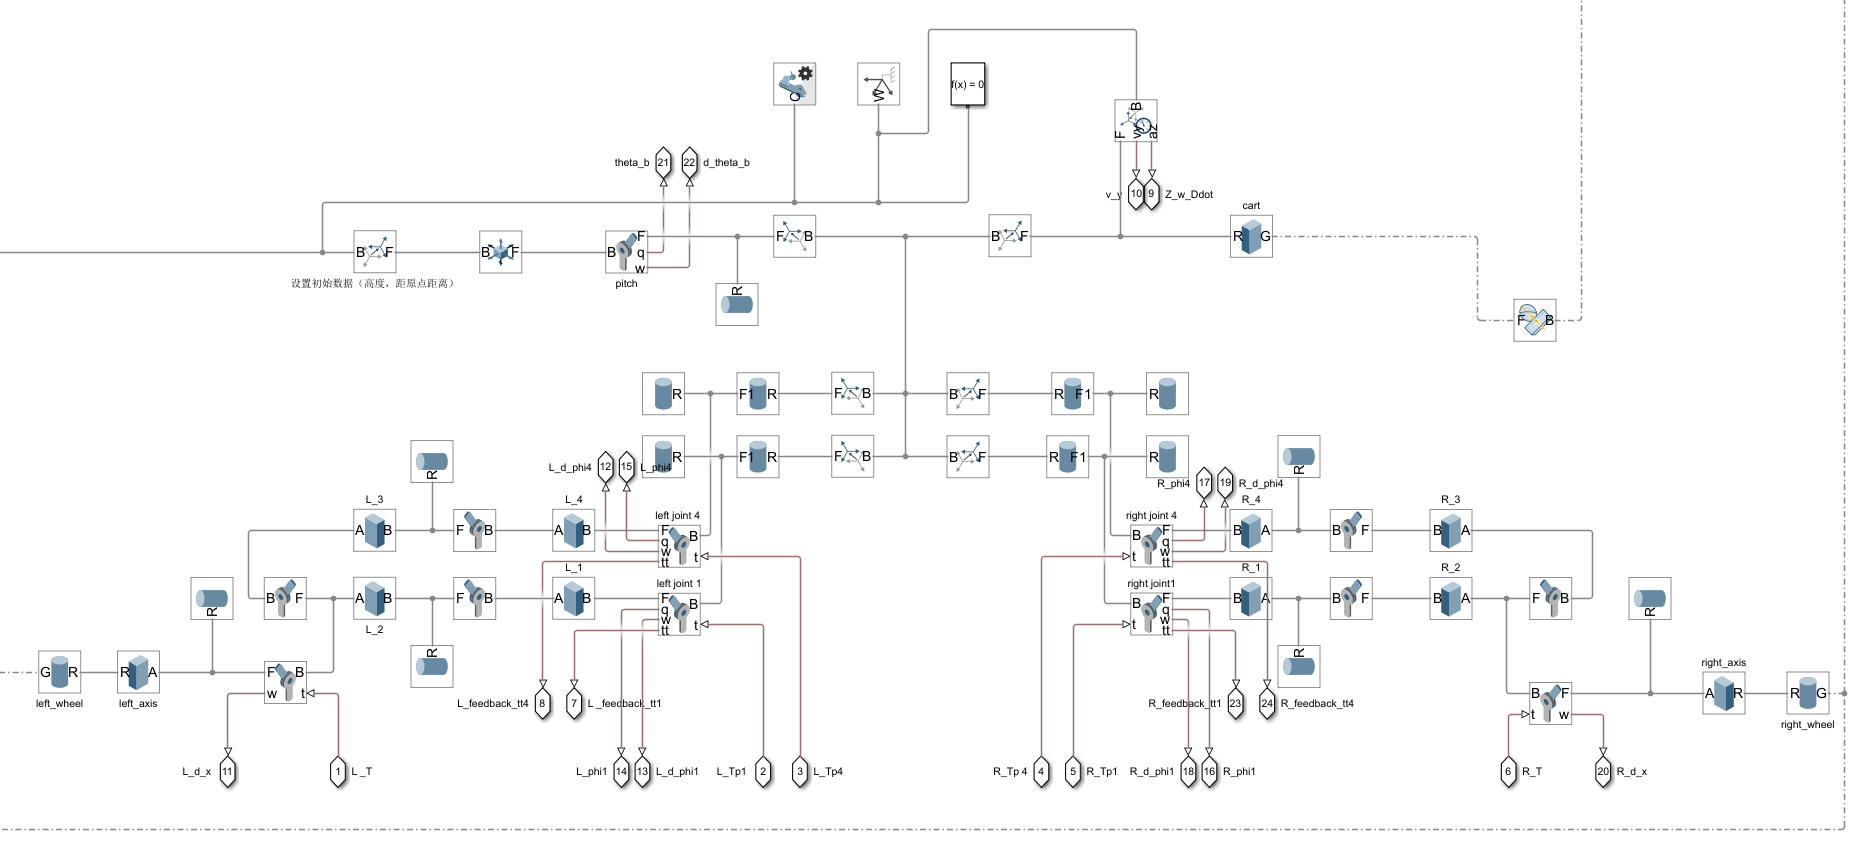
\includegraphics[width=0.7\textwidth]{figures/model_simulink_inside.png}
  \caption{轮腿机器人建模内部实现}
  \label{fig:model-simulink-inside}
\end{figure}

\begin{figure}[H]
  \centering
  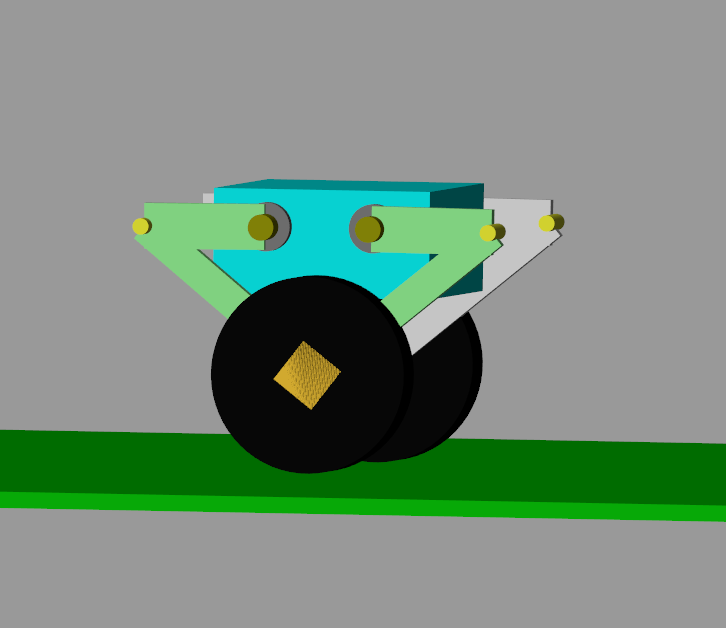
\includegraphics[width=0.5\textwidth]{figures/simulink_model.png}
  \caption{机器人建模}
  \label{fig:robot-model}
\end{figure}

\subsection{lqr控制模块}
\begin{figure}[H]
  \centering
  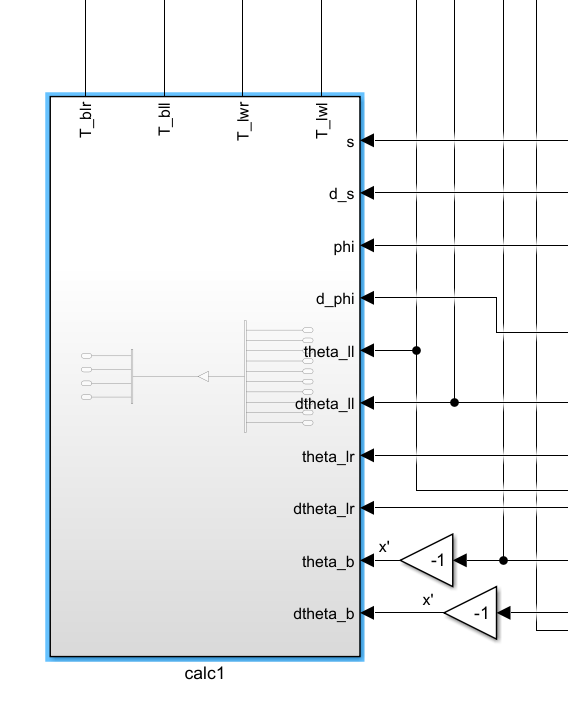
\includegraphics[width=0.3\textwidth]{figures/lqr_outside.png}
  \caption{lqr控制器外部接口}
  \label{fig:lqr-outside}
\end{figure}

\begin{figure}[H]
  \centering
  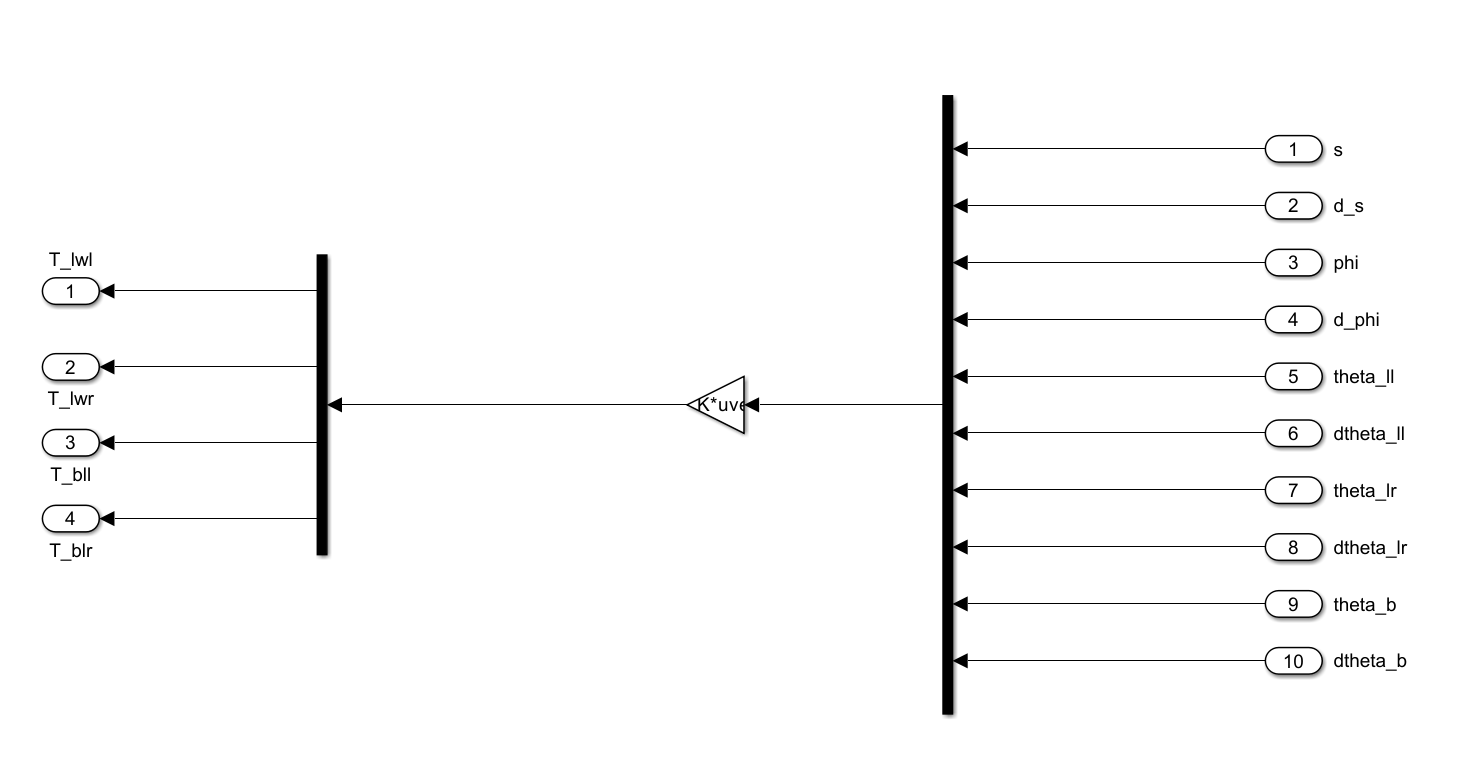
\includegraphics[width=0.9\textwidth]{figures/lqr_inside.png}
  \caption{lqr控制器内部实现}
  \label{fig:lqr-inside}
\end{figure}

LQR控制模块通过系统状态量的输入乘已经计算好的K矩阵该模块的输入包括机器人水平位移、水平位移速度、机器人yaw转角、yaw转角速度、腿部摆杆角度、腿部摆杆角速度、机体倾角、机体倾角速度状态量，输出腿部等效力矩和轮电机力矩。

\subsection{状态量求解与VMC}
\begin{figure}[H]
  \centering
  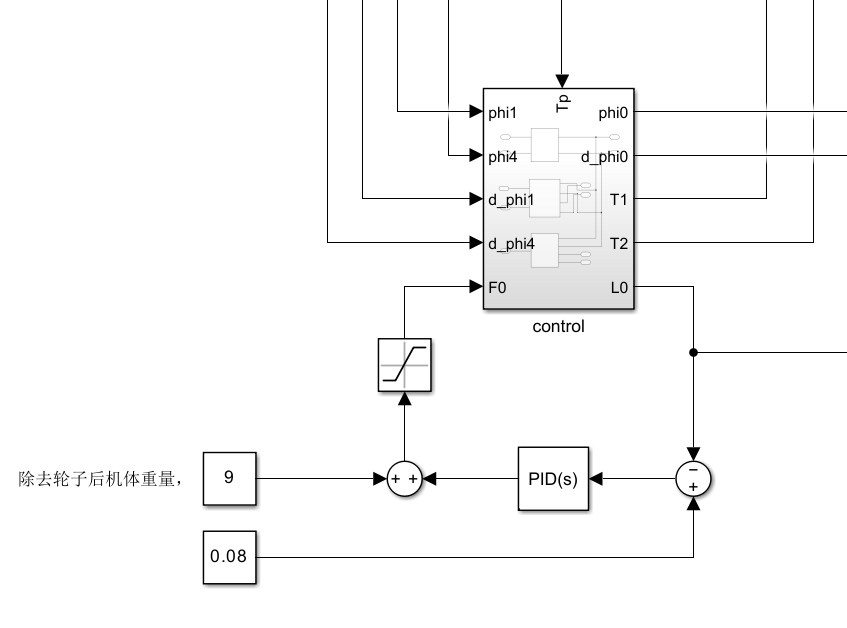
\includegraphics[width=0.5\textwidth]{figures/control_state_vmc_outside.png}
  \caption{状态量求解与VMC转化外部接口}
  \label{fig:state-and-vmc-outside}
\end{figure}

\begin{figure}[H]
  \centering
  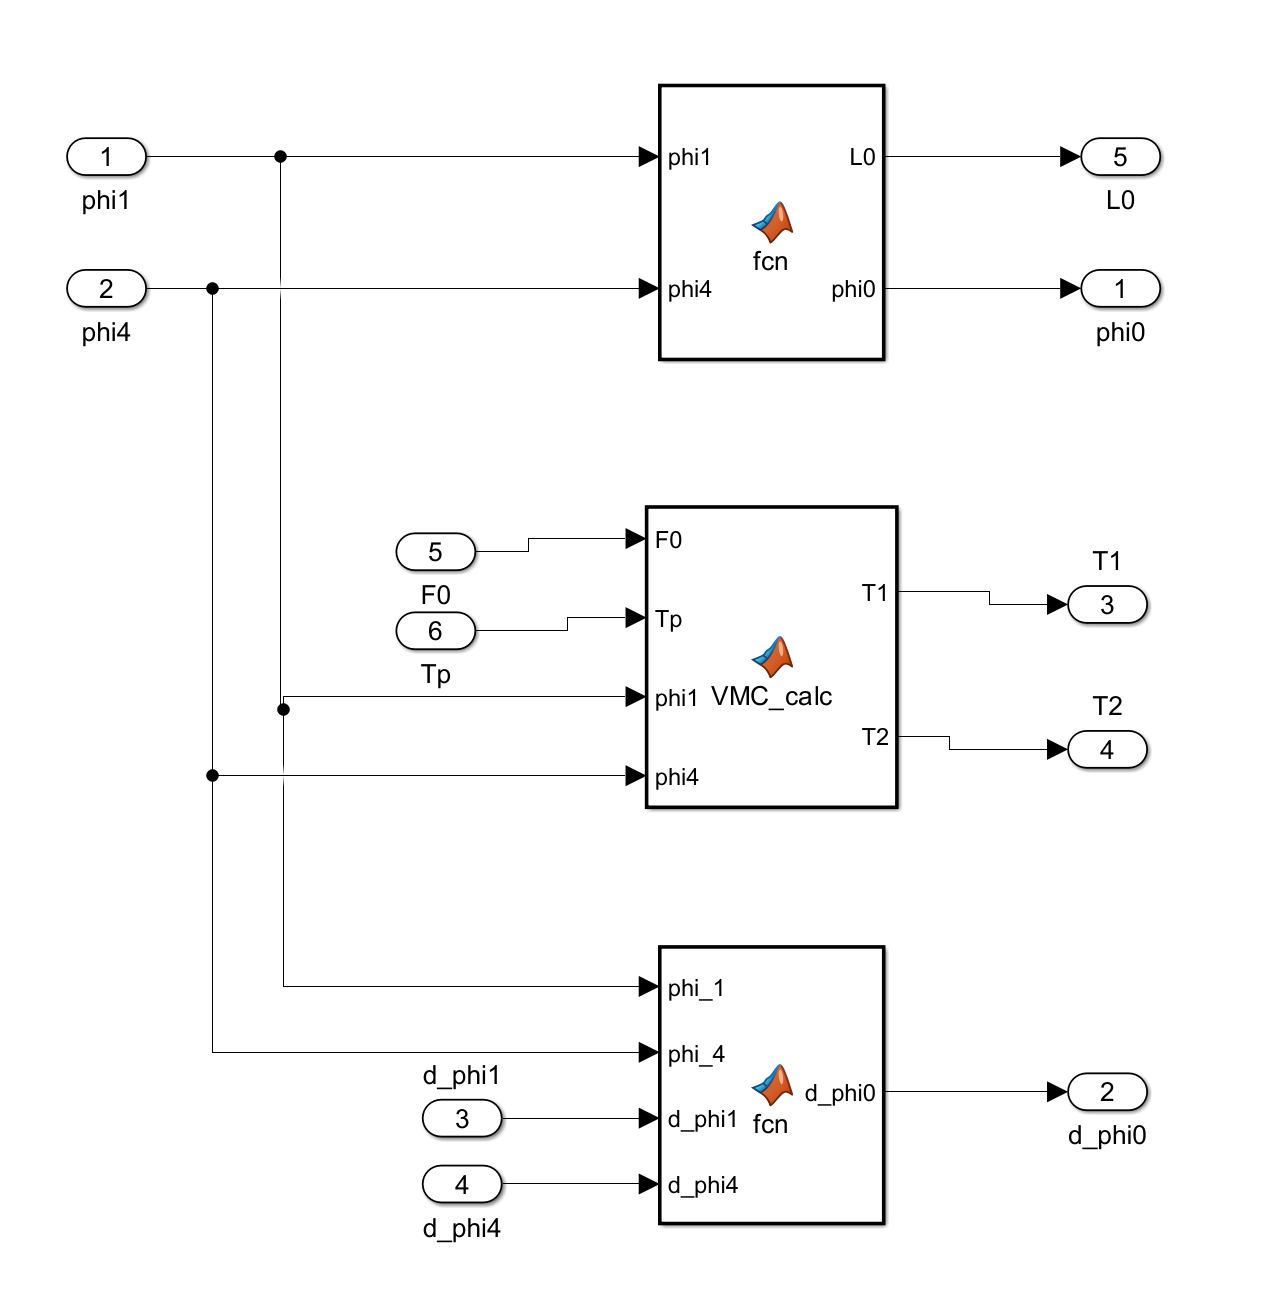
\includegraphics[width=0.5\textwidth]{figures/control_state_vmc_inside.png}
  \caption{状态量求解与VMC转化内部实现}
  \label{fig:state-and-vmc-inside}
\end{figure}

该模块的作用为通过 $\phi_1$、$\phi_4$，经过几何解算求得 $L_0$ 和 $\phi_0$，同时可再结合 $F_0$ 和 $T_p$ 通过 VMC 转化求得两个关节电机的控制输入。同时还通过雅各比矩阵求得 $\dot{\phi}_0$，便于后续继续求解腿角速度等。

\subsubsection{五连杆运动学解算}

\begin{minted}[breaklines,linenos,fontsize=\small]{matlab}
function [L0,phi0] = fcn(phi1,phi4)
   
    l5=0.08;%AE长度
    l1=0.075;
    l2=0.14;
    l3=0.14;
    l4=0.075;
    
    YD = l4*sin(phi4);
    YB = l1*sin(phi1);
    XD = l5 + l4*cos(phi4);
    XB = l1*cos(phi1); 
    lBD = sqrt((XD - XB)*(XD - XB) + (YD - YB)*(YD - YB));
    A0 = 2*l2*(XD - XB);
    B0 = 2*l2*(YD - YB);
    C0 = l2*l2 + lBD*lBD - l3*l3;
    phi2 = 2*atan2((B0 + sqrt(A0*A0 + B0*B0 - C0*C0)),(A0 + C0));
    XC = l1*cos(phi1) + l2*cos(phi2);
    YC = l1*sin(phi1) + l2*sin(phi2);
    L0 = sqrt((XC - l5/2)*(XC - l5/2) + YC*YC);
    phi0=atan2(YC,(XC-l5/2));
    
end
\end{minted}

\subsubsection{VMC解算}

\begin{minted}[breaklines,linenos,fontsize=\small]{matlab}
function [T1,T2] = VMC_calc(F0,Tp,phi1,phi4)

    l5=0.08;%AE长度
    l1=0.075;
    l2=0.14;
    l3=0.14;
    l4=0.075;

YD = l4*sin(phi4);
YB = l1*sin(phi1);
XD = l5 + l4*cos(phi4);
XB = l1*cos(phi1); 
lBD = sqrt((XD - XB)*(XD - XB) + (YD - YB)*(YD - YB));
A0 = 2*l2*(XD - XB);
B0 = 2*l2*(YD - YB);
C0 = l2*l2 + lBD*lBD - l3*l3;
phi2 = 2*atan2((B0 + sqrt(A0*A0 + B0*B0 - C0*C0)),A0 + C0);
phi3 = atan2(YB-YD+l2*sin(phi2),XB-XD+l2*cos(phi2));
XC = l1*cos(phi1) + l2*cos(phi2);
YC = l1*sin(phi1) + l2*sin(phi2);
L0 = sqrt((XC - l5/2)*(XC - l5/2) + YC*YC);
phi0 = atan2(YC,XC - l5/2);
j11 = (l1*sin(phi0-phi3)*sin(phi1-phi2))/sin(phi3-phi2);
j12 = (l1*cos(phi0-phi3)*sin(phi1-phi2))/(L0*sin(phi3-phi2));
j21 = (l4*sin(phi0-phi2)*sin(phi3-phi4))/sin(phi3-phi2);
j22 = (l4*cos(phi0-phi2)*sin(phi3-phi4))/(L0*sin(phi3-phi2));
J = [j11 j12; j21 j22];
F = [F0;Tp];
T = J * F;
T1 = T(1,1);
T2 = T(2,1);
end
\end{minted}

\subsubsection{不含机体倾角速度的腿角速度求解}

\begin{minted}[breaklines,linenos,fontsize=\small]{matlab}
function d_phi0 = fcn(phi_1, phi_4, d_phi1, d_phi4)
    % --- 几何参数 ---
    l5 = 0.08;  % 机身基座宽度 (AE)
    l1 = 0.075; % 主动臂1
    l2 = 0.14;  % 连杆2
    l3 = 0.14;  % 连杆3
    l4 = 0.075; % 主动臂4

    % --- 1. 正运动学求解 ---
    % A点在 (0,0), E点在 (l5, 0)
    % B点坐标 (主动臂1末端)
    xB = l1 * cos(phi_1);
    yB = l1 * sin(phi_1);
    
    % D点坐标 (主动臂4末端)
    xD = l5 + l4 * cos(phi_4);
    yD = l4 * sin(phi_4);

    % 求解 B, D 两圆交点 C (足端)
    distBD = sqrt((xD - xB)^2 + (yD - yB)^2);
    a = (l2^2 - l3^2 + distBD^2) / (2 * distBD);
    h = sqrt(max(0, l2^2 - a^2));
    
    x2 = xB + a * (xD - xB) / distBD;
    y2 = yB + a * (yD - yB) / distBD;
    
    % 足端 C 的坐标 
    xc = x2 + h * (yD - yB) / distBD;
    yc = y2 - h * (xD - xB) / distBD;

    % 计算被动段角度 phi2, phi3
    phi_2 = atan2(yc - yB, xc - xB);
    phi_3 = atan2(yc - yD, xc - xD);

    % --- 2. 雅可比矩阵求解 ---
    sin_diff = sin(phi_2 - phi_3);
    J11 = l1 * sin(phi_1 - phi_3) * cos(phi_2) / sin_diff; 
    J12 = l4 * sin(phi_4 - phi_2) * cos(phi_3) / sin_diff;
    J21 = l1 * sin(phi_1 - phi_3) * sin(phi_2) / sin_diff;
    J22 = l4 * sin(phi_4 - phi_2) * sin(phi_3) / sin_diff;
    
    dxc = J11 * d_phi1 + J12 * d_phi4;
    dyc = J21 * d_phi1 + J22 * d_phi4;

    % --- 3. 计算腿部摆动角速度 ---
    l02 = xc^2 + yc^2;    
    d_phi0 = (xc * dyc - yc * dxc) / l02;
end
\end{minted}

\section{仿真条件设置}

本仿真在MATLAB R2024a环境下进行，使用Simulink 10.0版本。仿真时间设置为10秒，求解器为ode45变步长。机器人初始状态设定为距离地面高度30cm处落下，随后在1s和5s时间点处给定速度激励1m/s和-1m/s。仿真场景包括前半段的平坦地面和连续四个高度为0.25米的障碍物，机器人需要从初始状态落下到起点并越过障碍物，期间保持机体稳定不发散。

控制器参数设置如下：LQR权重矩阵$Q$设定为对状态量的单位矩阵，控制输入权重矩阵$R$设定为对控制输入的单位矩阵。仿真过程中，机器人需要根据控制器输出的力矩调整轮电机和关节电机的输入，以实现稳定的运动控制。
\begin{minted}[breaklines,linenos,fontsize=\small]{matlab}
%        s     ds     phi     dphi     theta_ll dtheta_ll theta_lr dtheta_lr theta_b dtheta_b
lqr_Q = [10,    0,     0,      0,       0,       0,       0,      0,       0,       0;
         0,    5,     0,      0,       0,       0,        0,       0,        0,       0;
         0,    0,     10,      0,       0,       0,       0,      0,       0,       0;
         0,    0,     0,      5,       0,       0,        0,       0,        0,       0;
         0,    0,     0,      0,       1,       0,        0,       0,        0,       0;
         0,    0,     0,      0,       0,       0.07,     0,       0,        0,       0;
         0,    0,     0,      0,       0,       0,        1,       0,        0,       0;
         0,    0,     0,      0,       0,       0,        0,       0.07,     0,       0;
         0,    0,     0,      0,       0,       0,        0,       0,        10,       0;
         0,    0,     0,      0,       0,       0,        0,       0,        0,      0.6];
% 其中：
% s       : 自然坐标系下机器人水平方向移动距离，单位：m，ds为其导数
% phi     ：机器人水平方向移动时yaw偏航角度，dphi为其导数
% theta_ll：左腿摆杆与竖直方向（自然坐标系z轴）夹角，dtheta_ll为其导数
% theta_lr：右腿摆杆与竖直方向（自然坐标系z轴）夹角，dtheta_lr为其导数
% theta_b ：机体与自然坐标系水平夹角，dtheta_b为其导数

% 矩阵中，以下列分别对应：
%        T_wl    T_wr     T_bl     T_br
lqr_R = [20,      0,       0,       0;
         0,      20,       0,       0;
         0,      0,       10,       0;
         0,      0,       0,       10];
\end{minted}

\section{仿真结果分析}
\begin{figure}[H]
  \centering
  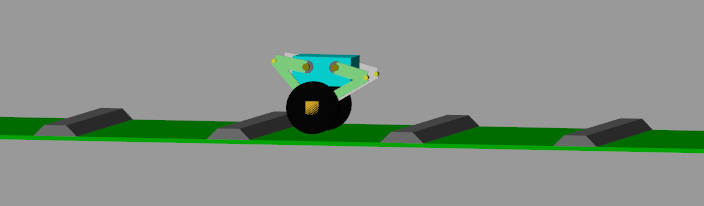
\includegraphics[width=0.5\textwidth]{figures/obstacle_1.png}
  \caption{越障前的机器人状态}
  \label{fig:obstacle-1}
\end{figure}
\begin{figure}[H]
  \centering
  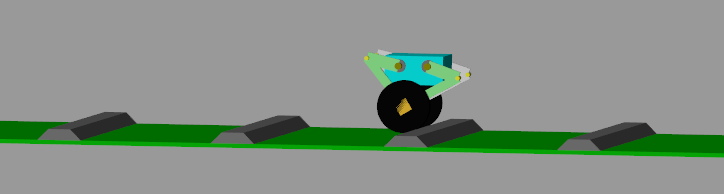
\includegraphics[width=0.5\textwidth]{figures/obstacle_2.png}
  \caption{越障中的机器人状态1}
  \label{fig:obstacle-2}
\end{figure}
\begin{figure}[H]
  \centering
  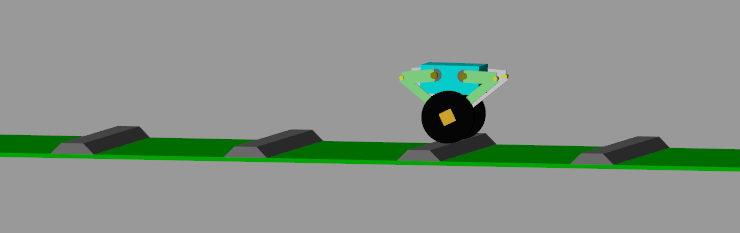
\includegraphics[width=0.5\textwidth]{figures/obstacle_3.png}
  \caption{越障中的机器人状态2}
  \label{fig:obstacle-3}
\end{figure}
\begin{figure}[H]
  \centering
  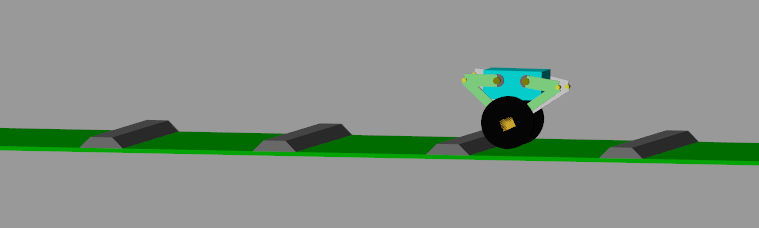
\includegraphics[width=0.5\textwidth]{figures/obstacle_4.png}
  \caption{越障后的机器人状态}
  \label{fig:obstacle-4}
\end{figure}


\section{仿真结果分析}
\begin{figure}[H]
  \centering
  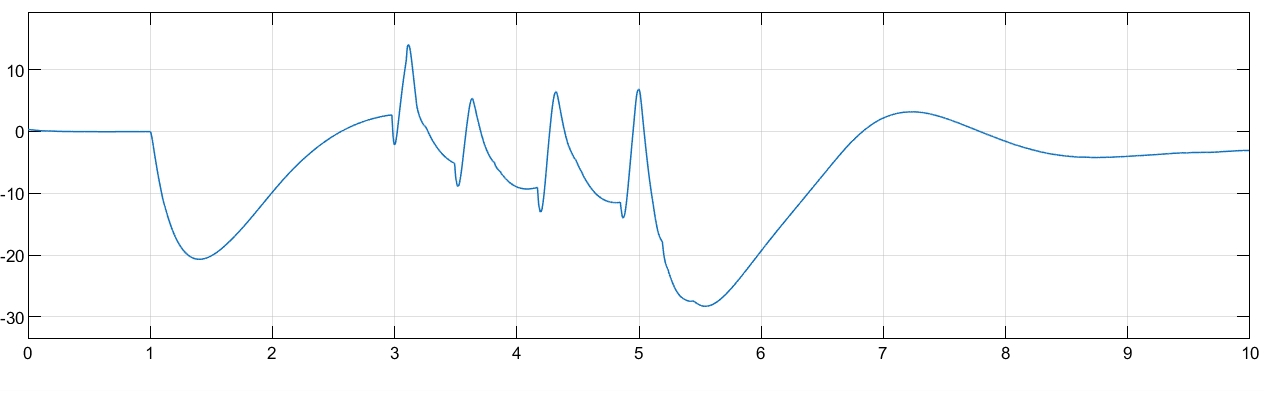
\includegraphics[width=0.5\textwidth]{figures/simulink_theta.png}
  \caption{状态量腿角度变化曲线}
  \label{fig:theta}
\end{figure}
\begin{figure}[H]
  \centering
  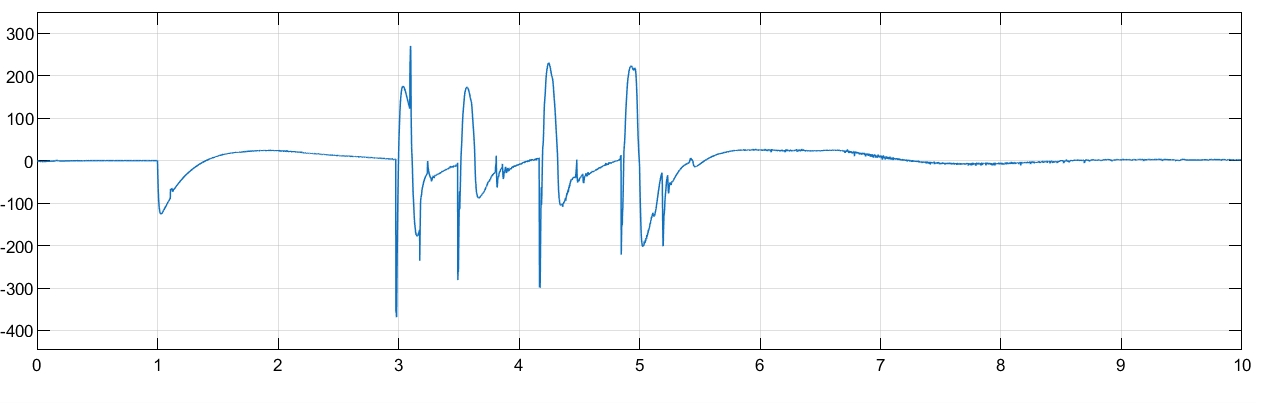
\includegraphics[width=0.5\textwidth]{figures/simulink_dtheta.png}
  \caption{状态量腿角速度变化曲线}
  \label{fig:dtheta}
\end{figure}
\begin{figure}[H]
  \centering
  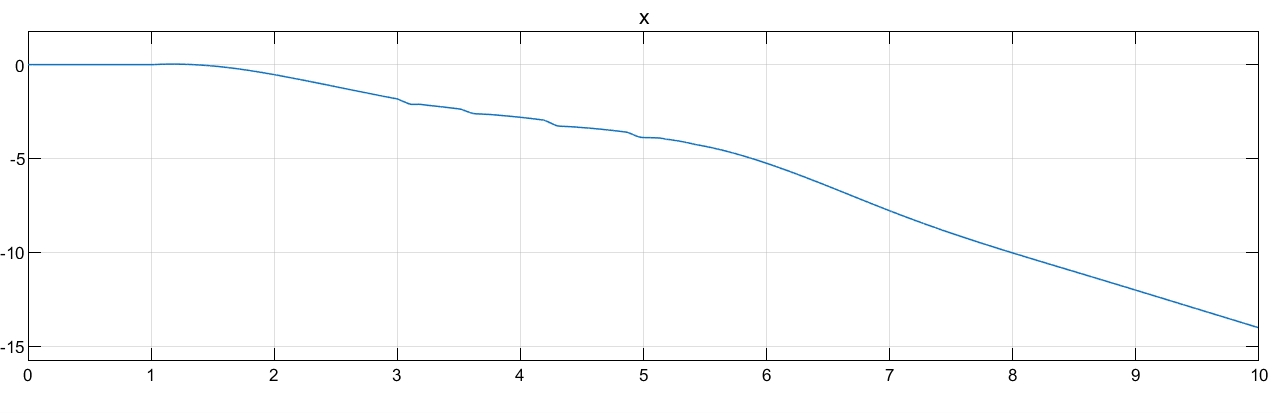
\includegraphics[width=0.5\textwidth]{figures/simulink_x.png}
  \caption{状态量机器人水平位移变化曲线}
  \label{fig:x}
\end{figure}
\begin{figure}[H]
  \centering
  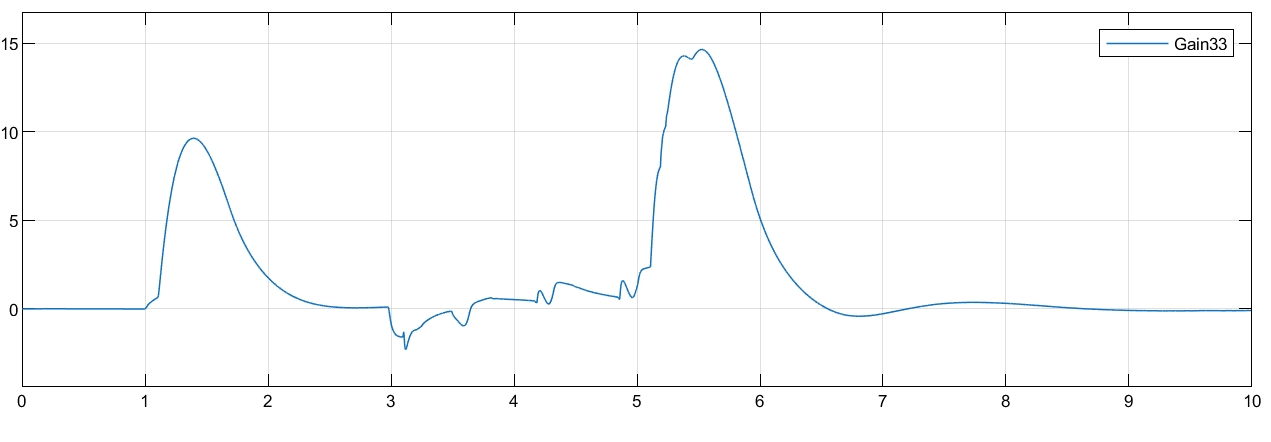
\includegraphics[width=0.5\textwidth]{figures/simulink_theta_b.png}
  \caption{状态量机体倾角变化曲线}
  \label{fig:theta_b}
\end{figure}
\begin{figure}[H]
  \centering
  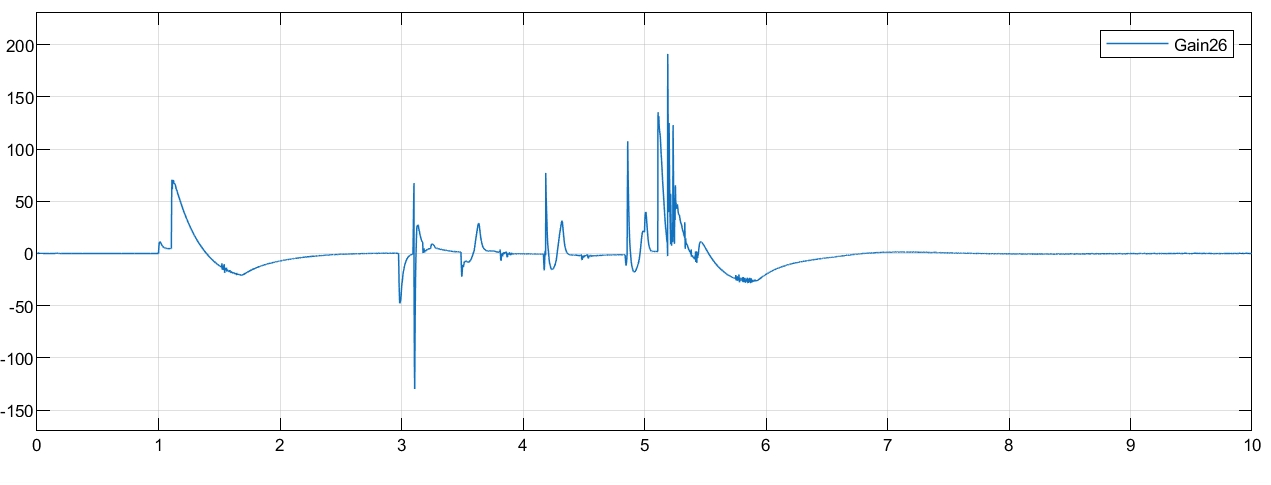
\includegraphics[width=0.5\textwidth]{figures/simulink_dtheta_b.png}
  \caption{状态量机体倾角速度变化曲线}
  \label{fig:dtheta_b}
\end{figure}
由此可见，机器人能够成功地越过障碍物，并且在整个过程中保持稳定的姿态和运动轨迹。这表明我们设计的控制方案在仿真环境中是有效的，能够实现预期的运动控制目标。

\begin{figure}[H]
  \centering
  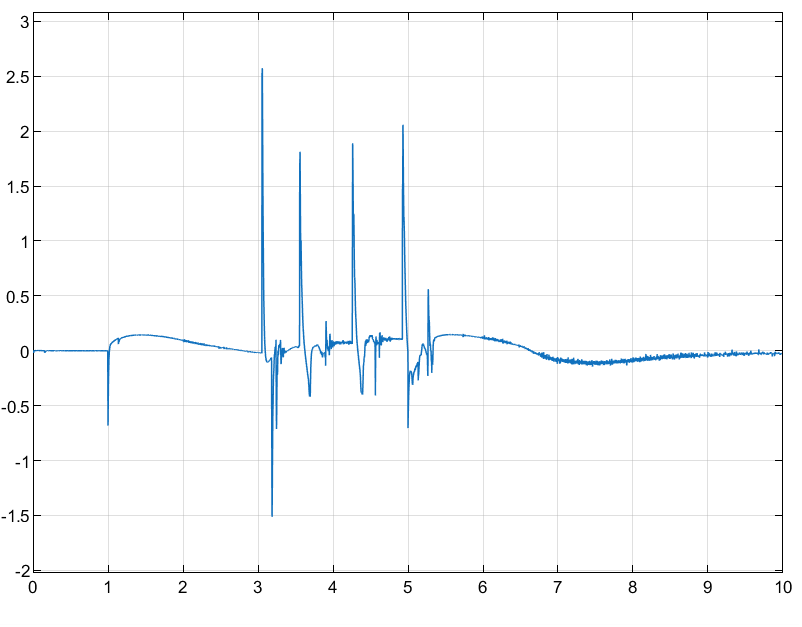
\includegraphics[width=0.7\textwidth]{figures/control_l_t.png}
  \caption{越障中的轮电机输出力矩}
  \label{fig:torque_wheel}
\end{figure}
\begin{figure}[H]
  \centering
  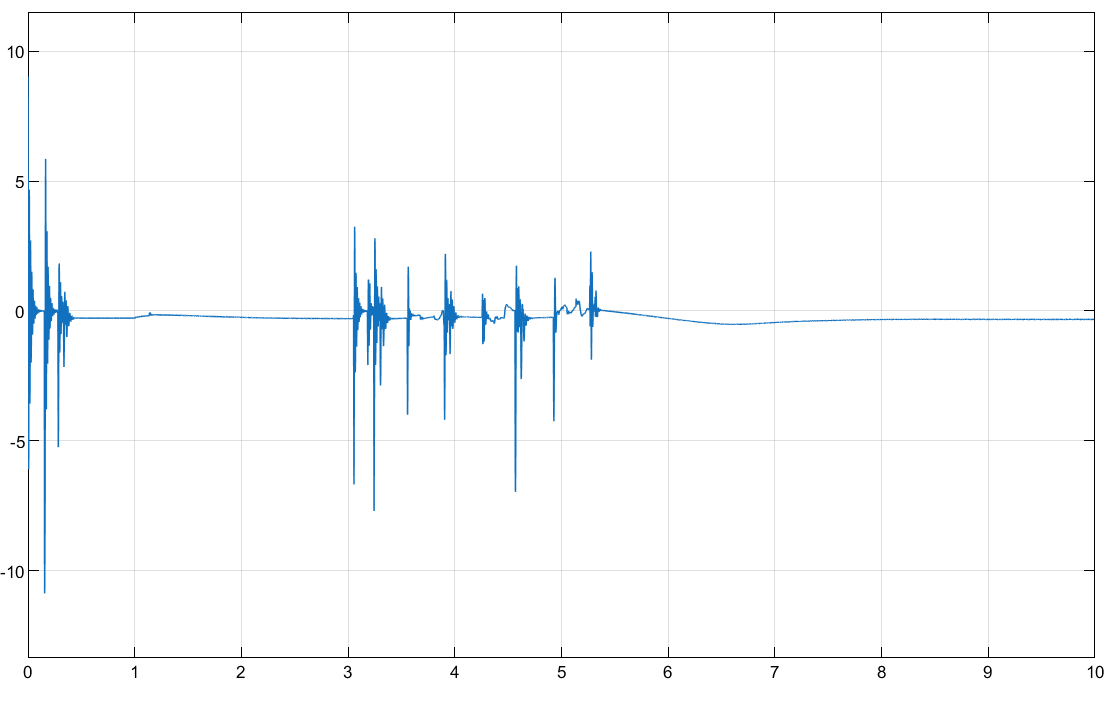
\includegraphics[width=0.7\textwidth]{figures/control_l_t1.png}
  \caption{越障中的前关节电机输出力矩}
  \label{fig:torque_joint_front}
\end{figure}
\begin{figure}[H]
  \centering
  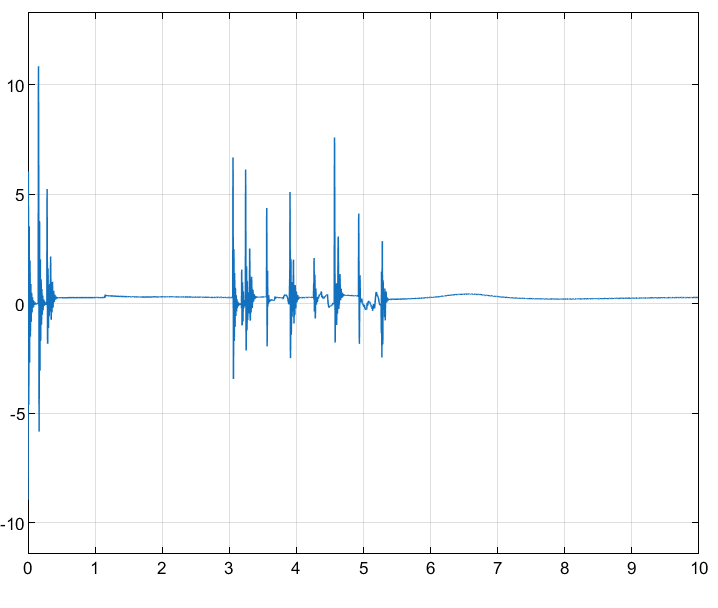
\includegraphics[width=0.7\textwidth]{figures/control_l_t4.png}
  \caption{越障中的后关节电机输出力矩}
  \label{fig:torque_joint_back}
\end{figure}

此外，我们再对越障过程中机器人的轮电机、关节电机输出进行分析，结果如图\ref{fig:torque_wheel}、\ref{fig:torque_joint_front}和\ref{fig:torque_joint_back}所示。可以看出，在越障过程中，轮电机和关节电机的输出都发生了明显的变化，以适应不同阶段的运动需求，但未达到饱和，且最终趋于稳定，这进一步验证了我们设计的控制方案能够根据环境变化动态调整控制输入，从而实现稳定的运动控制。
